\documentclass[a4paper,12pt]{article}
\usepackage[spanish]{babel}
\usepackage[utf8]{inputenc}
\usepackage[dvips]{graphicx}
\usepackage[dvips]{epsfig}
\usepackage[T1]{fontenc}

\newcommand{\PI}{{$\pi$ }}

\title{Número PI}
\author{María Pérez}
\date{10 de abril de 2014}

\begin{document}
\maketitle

\begin{abstract}
El número \PI se obtiene de la relación entre la longitud de una circunferencia y su diámetro, en geometría euclidia. Es un número irracional y una de las constantes matemáticas más importantes. Se emplea frecuentemente en matemáticas,física e ingeniería.
\cite{wikipedia}
\end{abstract}

\section{Motivación y Objetivos}
La principal motivación de este artículo es tener un mayor conocimiento sobre qué es el número PI, así mismo el objetivo es que el lector consiga tener una visión más clara de qué es el número PI.

\section{Número \PI}
\subsection{Introducción}
El número PI, representado por la letra griega \PI, equivale a la constante que relaciona el perímetro o longitud de una circunferencia con su diámetro. Se trata de un valor con un infinito número de decimales, cuya secuencia comienza de la siguiente manera:3,1415926535897932384626433832795028841…
Redondeado en 3,1416, pi es un número irracional -no puede representarse de forma fraccional-.
Al cálculo de pi se han dedicado millones de horas desde que los antiguos egipcios, allá por el año 1600 a.C, ya concluyeran que existía relación entre la longitud y el diámetro de una circunferencia.
Griegos tan insignes como Arquímedes o Ptolomeo experimentaron con polígonos de cientos de lados y circunferencias de decenas de unidades de radio para aproximarse al número pi con la mayor precisión posible. También lo hicieron en China e India, y más tarde en Europa, continente en el que el francés Fabrice Bellard, a principios de 2010, consiguió establecer el record de decimales conocidos de pi en 2,7 billones.
\subsection{Uso}
\PI es ubicuo\footnote{Qué está presente en todas partes, omnipresente} en matemática; aparece incluso en lugares que carecen de una conexión directa con los círculos de la geometría euclídea.
El uso más frecuente de \PI se da en geometría y trigonometría, en física, en análisis superior y teoría de números, em probabilidad y estadística (veáse la figura \ref{num_pi}


\begin{figure}[!th]
\begin{center}
\includegraphics[width=0.25\textwidth]{images/figura2.eps}
\caption{Número PI}
\label{num_pi}
\end{center}
\end{figure}

\begin{table}[!ht]
\begin{tabular}{|l|c|c|}
\hline
Nombre & Año & Aproximación\\ \hline
Papiro de Almes & 1650 a.C. & 3.16\\ \hline
Bandhayana & 500 a.C. & 3.09\\ \hline
Liu Hui & 260 d.C. & 3.1416\\ \hline
\end{tabular}
\cite{educacion}
\caption{Aproximaciones en la historia}
\label{tabla}
\end{table}

\begin{thebibliography}{00}
\bibliography{bib/references}
\end{thebibliography}

\end{document}  

          
 
